%% Autonomous end-to-end pipeline block diagram (fig:autonomous_pipeline).
%% Colour code: red = trained in this work (frozen at inference),
%% blue = external pre-trained (frozen), grey = deterministic (no learned parameters).
%% Matches the caption in chapter3_integration.tex.
%% Build: pdflatex autonomous_pipeline.tex; output copied to ../autonomous_pipeline.pdf
\documentclass[10pt,tikz,border=4pt]{standalone}
\usepackage[T1]{fontenc}
\usepackage{mathptmx}
\usepackage{amsmath,amssymb}
\usetikzlibrary{positioning,arrows.meta,calc}

\begin{document}
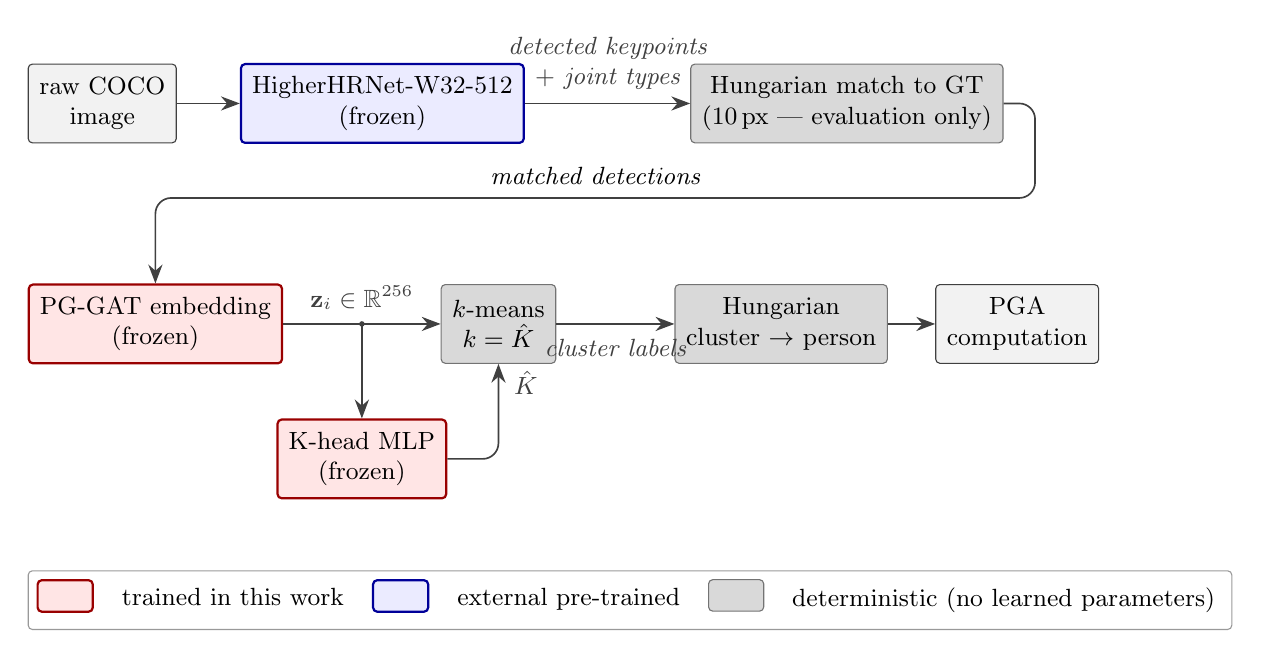
\begin{tikzpicture}[
  font=\small,
  >={Stealth[length=2.4mm]},
  box/.style={draw=black!75, rounded corners=1.5pt, align=center,
              inner sep=4pt, minimum height=10mm, fill=white},
  data/.style={box, fill=black!5},
  ours/.style={box, draw=red!60!black, fill=red!10, thick},
  ext/.style={box, draw=blue!60!black, fill=blue!8, thick},
  det/.style={box, draw=black!55, fill=black!15},
  arr/.style={->, semithick, black!75},
  dlbl/.style={font=\small\itshape, align=center},
]

%% ---------- row 1: detection and matching ----------
\node[data] (img) {raw COCO\\ image};

\node[ext, right=8mm of img] (hrnet) {HigherHRNet-W32-512\\ (frozen)};

\node[det, right=21mm of hrnet] (gtmatch) {Hungarian match to GT\\ (10\,px --- evaluation only)};

\draw[arr] (img) -- (hrnet);
\draw[arr] (hrnet) -- node[dlbl, above=0.5mm]{detected keypoints\\ $+$ joint types} (gtmatch);

%% ---------- elbow down to row 2 ----------
\node[ours, below=28mm of img.west, anchor=west] (pggat) {PG-GAT embedding\\ (frozen)};

\coordinate (c1) at ($(gtmatch.east)+(4mm,0)$);
\coordinate (c2) at ($(c1)+(0,-12mm)$);
\coordinate (c3) at (pggat.north |- c2);
\draw[arr, rounded corners=2mm] (gtmatch.east) -- (c1) -- (c2) -- (c3) -- (pggat.north);
\node[dlbl, above=0.5mm] at ($(c2)!0.5!(c3)$) {matched detections};

%% ---------- row 2: embedding, K estimation, grouping ----------
\node[det, right=20mm of pggat] (kmeans) {$k$-means\\ $k = \hat{K}$};

\node[det, right=15mm of kmeans] (hung) {Hungarian\\ cluster $\to$ person};

\node[data, right=6mm of hung] (pga) {PGA\\ computation};

\coordinate (branch) at ($(pggat.east)!0.5!(kmeans.west)$);
\node[ours, below=12mm of branch, anchor=north] (khead) {K-head MLP\\ (frozen)};

\draw[arr] (pggat) -- node[dlbl, above=0.5mm]{$\mathbf{z}_i \in \mathbb{R}^{256}$} (kmeans);
\fill[black!75] (branch) circle (1pt);
\draw[arr] (branch) -- (khead.north);
\draw[arr, rounded corners=2mm] (khead.east) -| node[dlbl, pos=0.9, right=0.7mm]{$\hat{K}$} (kmeans.south);

\draw[arr] (kmeans) -- node[dlbl, below=0.7mm]{cluster labels} (hung);
\draw[arr] (hung) -- (pga);

%% ---------- legend ----------
\matrix[draw=black!40, rounded corners=1.5pt, inner sep=3pt, column sep=2.5mm, row sep=1mm,
        ampersand replacement=\&] (leg)
        at ($(pggat.west |- khead.south)+(0,-9mm)$) [anchor=north west] {
  \node[ours, minimum height=4mm, minimum width=7mm, inner sep=1pt] {}; \&
  \node[align=left]{trained in this work}; \&
  \node[ext, minimum height=4mm, minimum width=7mm, inner sep=1pt] {}; \&
  \node[align=left]{external pre-trained}; \&
  \node[det, minimum height=4mm, minimum width=7mm, inner sep=1pt] {}; \&
  \node[align=left]{deterministic (no learned parameters)}; \\
};

\end{tikzpicture}
\end{document}
